\documentclass[12pt,letterpaper]{article}
\usepackage[utf8]{inputenc}
\usepackage[spanish]{babel}
\usepackage{graphicx}
\usepackage[left=2cm,right=2cm,top=2cm,bottom=2cm]{geometry}
\usepackage{graphicx} % figuras
% \usepackage{subfigure} % subfiguras
\usepackage{float} % para usar [H]
\usepackage{amsmath}
%\usepackage{txfonts}
\usepackage{stackrel} 
\usepackage{multirow}
\usepackage{enumerate} % enumerados
\renewcommand{\labelitemi}{$-$}
\renewcommand{\labelitemii}{$\cdot$}
% \author{}
% \title{Caratula}
\begin{document}

% Fancy Header and Footer
% \usepackage{fancyhdr}
% \pagestyle{fancy}
% \cfoot{}
% \rfoot{\thepage}
%

% \usepackage[hidelinks]{hyperref} % CREA HYPERVINCULOS EN INDICE

% \author{}
\title{Caratula}

\begin{titlepage}
\begin{center}
\large{UNERSIDAD PRIVADA DE TACNA}\\
\vspace*{-0.025in}
\begin{figure}[htb]
\begin{center}

\includegraphics[width=8cm]{./images/logo}
\end{center}
\end{figure}
\vspace*{0.15in}
INGENIERIA DE SISTEMAS  \\

\vspace*{0.5in}
\begin{large}
TITULO:\\
\end{large}

\vspace*{0.1in}
\begin{Large}
\textbf{INFORME DE LABORATORIO N 05} \\
\end{Large}

\vspace*{0.3in}
\begin{Large}
\textbf{CURSO:} \\
\end{Large}

\vspace*{0.1in}
\begin{large}
BASE DE DATOS II\\
\end{large}

\vspace*{0.3in}
\begin{Large}
\textbf{DOCENTE(ING):} \\
\end{Large}

\vspace*{0.1in}
\begin{large}
 Patrick Cuadros Quiroga\\
\end{large}

\vspace*{0.2in}
\vspace*{0.1in}
\begin{large}
Integrantes: \\
\begin{flushleft}
Moreno Mulluni Luis Angel		\hfill	(2017057864) \\
Layme Valeriano Diego 		\hfill	(2017057865) \\
Mamani Calisaya Yonathan 	           	\hfill	(2017057863) \\
\end{flushleft}
\end{large}
\end{center}

\end{titlepage}


\tableofcontents % INDICE
\thispagestyle{empty} % INDICE SIN NUMERO
\newpage
\setcounter{page}{1} % REINICIAR CONTADOR DE PAGINAS DESPUES DEL INDICE

\section{Actividad N 01 – Valores} 
\textbf{Los valores introducidos al archivo sysctl.conf ¿que representan?}

\begin{flushleft}
El comando sysctl es usado para visualizar, configurar y automatizar configuraciones del kernel en el directorio.
\end{flushleft}

\begin{itemize}
	\item \textbf{fs.suid\_dumpable}

	\begin{flushleft}
	\textbf{Desactivación de volcados de núcleo}\\
Por defecto, el sistema previene setuidy los setgid programas, los programas que han cambiado las credenciales y los programas cuyos binarios no tienen permiso de lectura del núcleo de volcado. Para asegurarse de que la configuración se registra de forma permanente, agregue las siguientes líneas a /etc/sysctl.conf:\\
\vspace{5mm} %5mm vertical space
	\# No permitir el volcado de núcleo por los programas setuid y setgid\\
	fs.suid\_dumpable = 0\\
\vspace{5mm}
	y luego ejecute el comando sysctl -p\\
\vspace{5mm} %5mm vertical space
\textbf{Nota}\\
Un valor de 1 permite volcados de núcleo que pueden ser leídos por el propietario del proceso de dumping. Un valor de 2 permite volcados de núcleo que solo se pueden leer con rootfines de depuración.
	\end{flushleft}

	\item \textbf{fs.aio-max-nr}

\begin{flushleft}
\textbf{Asegurando un rendimiento predecible}\\
El kernel de Linux proporciona la función de E / S sin bloqueo asíncrono (AIO) que permite que un proceso inicie varias operaciones de E / S simultáneamente sin tener que esperar a que se complete ninguna de ellas. Esto ayuda a mejorar el rendimiento de las aplicaciones que pueden solapar el procesamiento y la E / S.\\
\vspace{5mm} 
aio-max-nr parámetro que determina el número máximo de solicitudes concurrentes permitidas.\\
\vspace{5mm}
Se recomienda que establezca el aio-max-nrvalor en 1048576. Esto ayuda a HyperScale a tener un rendimiento óptimo, en un entorno que involucra grandes cargas de trabajo de E / S.\\
\vspace{5mm}
Realice los siguientes pasos en todos los nodos de cómputo y datos de HyperScale:
\begin{enumerate}
\item Para establecer el aio-max-nr, agregue la siguiente línea al /etc/sysctl.conf\\
fs.aio-max-nr = 1048576
\item Para activar la nueva configuración, ejecute el siguiente comando\\
\# sysctl -p /etc/sysctl.conf
\end{enumerate}
\end{flushleft}


	\item \textbf{fs.file-max}

\begin{flushleft}
\textbf{Número máximo de manejadores de archivos}\\
El número máximo de identificadores de archivos denota el número máximo de archivos abiertos en un sistema Linux.\\
\vspace{5mm}
Oracle recomienda que los manejadores de archivos para todo el sistema estén configurados en al menos 65536 para 9i R2 y 10g R1 y R2 para plataformas x86 y x86-64.\\
\vspace{5mm}
Edite el archivo /etc/sysctl.conf y agregue la siguiente línea:\\
\# Mejorar el número de archivos abiertos.\\
fs.file-max = 6815744\\
\end{flushleft}


	\item \textbf{kernel.shmmni}


\begin{flushleft}
\textbf{Parámetro SHMMNI}\\
Este parámetro establece el número máximo de segmentos de memoria compartida en todo el sistema.\\
\vspace{5mm}
Oracle recomienda que SHMMNI sea al menos 4096 para Oracle 10g. Para Oracle 9i en x86, la configuración mínima recomendada es menor. Dado que estas recomendaciones son configuraciones mínimas, es mejor establecerlas siempre en al menos 4096 para las bases de datos 9i y 10g en las plataformas x86 y x86-64.\\
\vspace{5mm}
Edite el archivo /etc/sysctl.conf y agregue la siguiente línea:\\
kernel.shmmni = 4096\\
\end{flushleft}


	\item \textbf{kernel.sem}

\begin{flushleft}
\textbf{Parámetros de Semáforo}\\
Los semáforos son un recurso que se puede compartir y que toman un valor entero no negativo. Están manipulados por las funciones P (esperar) y V (señal), que disminuyen e incrementan el semáforo, respectivamente. Cuando un proceso necesita un recurso, se emite una "espera" y se disminuye el semáforo. Cuando el semáforo contiene un valor de cero, los recursos no están disponibles y el proceso de llamada gira o se bloquea (según corresponda) hasta que los recursos estén disponibles. Cuando un proceso libera un recurso controlado por un semáforo, incrementa el semáforo y se notifica a los procesos en espera.\\
\vspace{5mm}
Edite el archivo /etc/sysctl.conf y agregue la siguiente línea:\\
\# semáforos: semmsl, semmns, semopm, semmni\\
kernel.sem = 250 32000 100 128\\
\vspace{5mm}
Estos valores representan SEMMSL, SEMMNS, SEMOPM y SEMMNI.
\begin{enumerate}
\item \textbf{SEMMSL} Número máximo de semáforos por matriz (mínimo 128)
\item \textbf{SEMMNS} semáforos máximos en todo el sistema
\item \textbf{SEMOPM} operaciones máximas por llamada semop
\item \textbf{SEMMNI} matrices máximas
\end{enumerate}
\end{flushleft}


	\item \textbf{net.ipv4.ip\_local\_port\_range}

\begin{flushleft}
\textbf{Rango de Puertos}\\
Para servidores de red con mucho tráfico, como servidores proxy o balanceadores de carga, es posible que deba aumentar el rango de puertos de red.\\
\vspace{5mm}
ip\_local\_port\_range que define el puerto mínimo y máximo que una conexión de red puede usar como su puerto de origen (local). Esto se aplica a las conexiones TCP (Protocolo de Control de Transmisión) y UDP (Protocolo de datagramas de usuario).\\
\vspace{5mm}
Edite el archivo /etc/sysctl.conf y agregue la siguiente línea:\\
net.ipv4.ip\_local\_port\_range = 9000 65500\\
\vspace{5mm}
El primer número es el primer puerto local permitido para el tráfico TCP y UDP, y el segundo número es el último número de puerto.\\
\end{flushleft}

\item \textbf{Sintonización de red / TCP / UDP}

\begin{flushleft}
Esta es una descripción muy básica paso a paso de cómo mejorar el rendimiento de las redes (TCP y UDP) en Linux 2.4+ para aplicaciones de alto ancho de banda. Estas configuraciones son especialmente importantes para los enlaces GigE (Gigabit Ethernet).\\
\end{flushleft}

\begin{itemize}
	\item \textbf{net.core.rmem\_default}

\begin{flushleft}
Esto establece el tamaño predeterminado del búfer de recepción del sistema operativo para todos los tipos de conexiones.\\
\vspace{5mm}
net.core.rmem\_default=262144\\
\end{flushleft}

	\item \textbf{net.core.rmem\_max}

\begin{flushleft}
Esto establece el tamaño máximo del búfer de recepción del SO para todos los tipos de conexiones.\\
\vspace{5mm}
net.core.rmem\_max=4194304\\
\end{flushleft}

	\item \textbf{net.core.wmem\_default}

\begin{flushleft}
Esto establece el tamaño máximo del búfer de envío del sistema operativo para todos los tipos de conexiones.\\
\vspace{5mm}
net.core.wmem\_default=262144\\
\end{flushleft}

	\item \textbf{net.core.wmem\_max}

\begin{flushleft}
Esto establece el tamaño máximo del búfer de envío del sistema operativo para todos los tipos de conexiones.\\
\vspace{5mm}
net.core.wmem\_max=4194304\\
\end{flushleft}

\end{itemize}


\end{itemize}

\section{Actividad N 02 – Usuarios} 
\textbf{¿Con qué usuario(s) puedo conectarme al servidor a través del Administrador
Empresarial?}\\
\begin{flushleft}
Con el usuario: \textbf{SYS}\\
\end{flushleft}
\section{Actividad N 03 – Administrador Empresarial} 
\textbf{Capture una imagen de pantalla del navegador con el Administrador Empresarial, con el nombre de su servidor e iniciada la sesión del usuario SYS.}
\vspace{5mm}
\begin{center}
  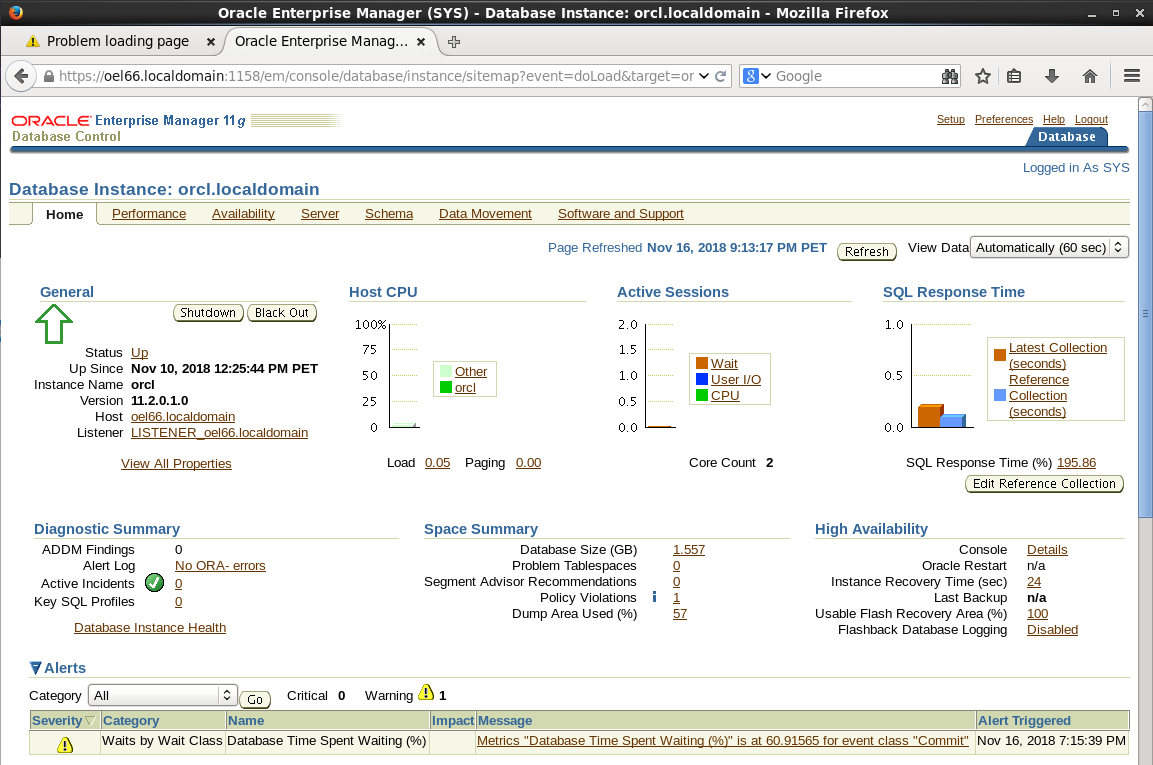
\includegraphics[width=\columnwidth]{images/admi-empresarial}\\
\end{center}


\end{document}